\documentclass[11pt]{article}

\usepackage[UTF8]{ctex} % for Chinese 
\setCJKmainfont[ItalicFont=Noto Sans CJK SC Bold, BoldFont=Noto Serif CJK SC Black]{Noto Serif CJK SC} % for Chinese

\usepackage{setspace}
\usepackage[colorlinks,linkcolor=blue,anchorcolor=red,citecolor=black]{hyperref}
\usepackage{lineno}
\usepackage{booktabs}
\usepackage{graphicx}
\usepackage{float}
\usepackage{floatrow}
\usepackage{subfigure}
\usepackage{caption}
\usepackage{subcaption}
\usepackage{geometry}
\usepackage{multirow}
\usepackage{longtable}
\usepackage{lscape}
\usepackage{booktabs}
\usepackage{natbib}
\usepackage{natbibspacing}
\usepackage[toc,page]{appendix}
\usepackage{makecell}

\title{庄子}
\date{}

\linespread{1.5}
\geometry{left=2cm,right=2cm,top=2cm,bottom=2cm}

\begin{document}

  \maketitle

  \begin{figure}
    \centering
    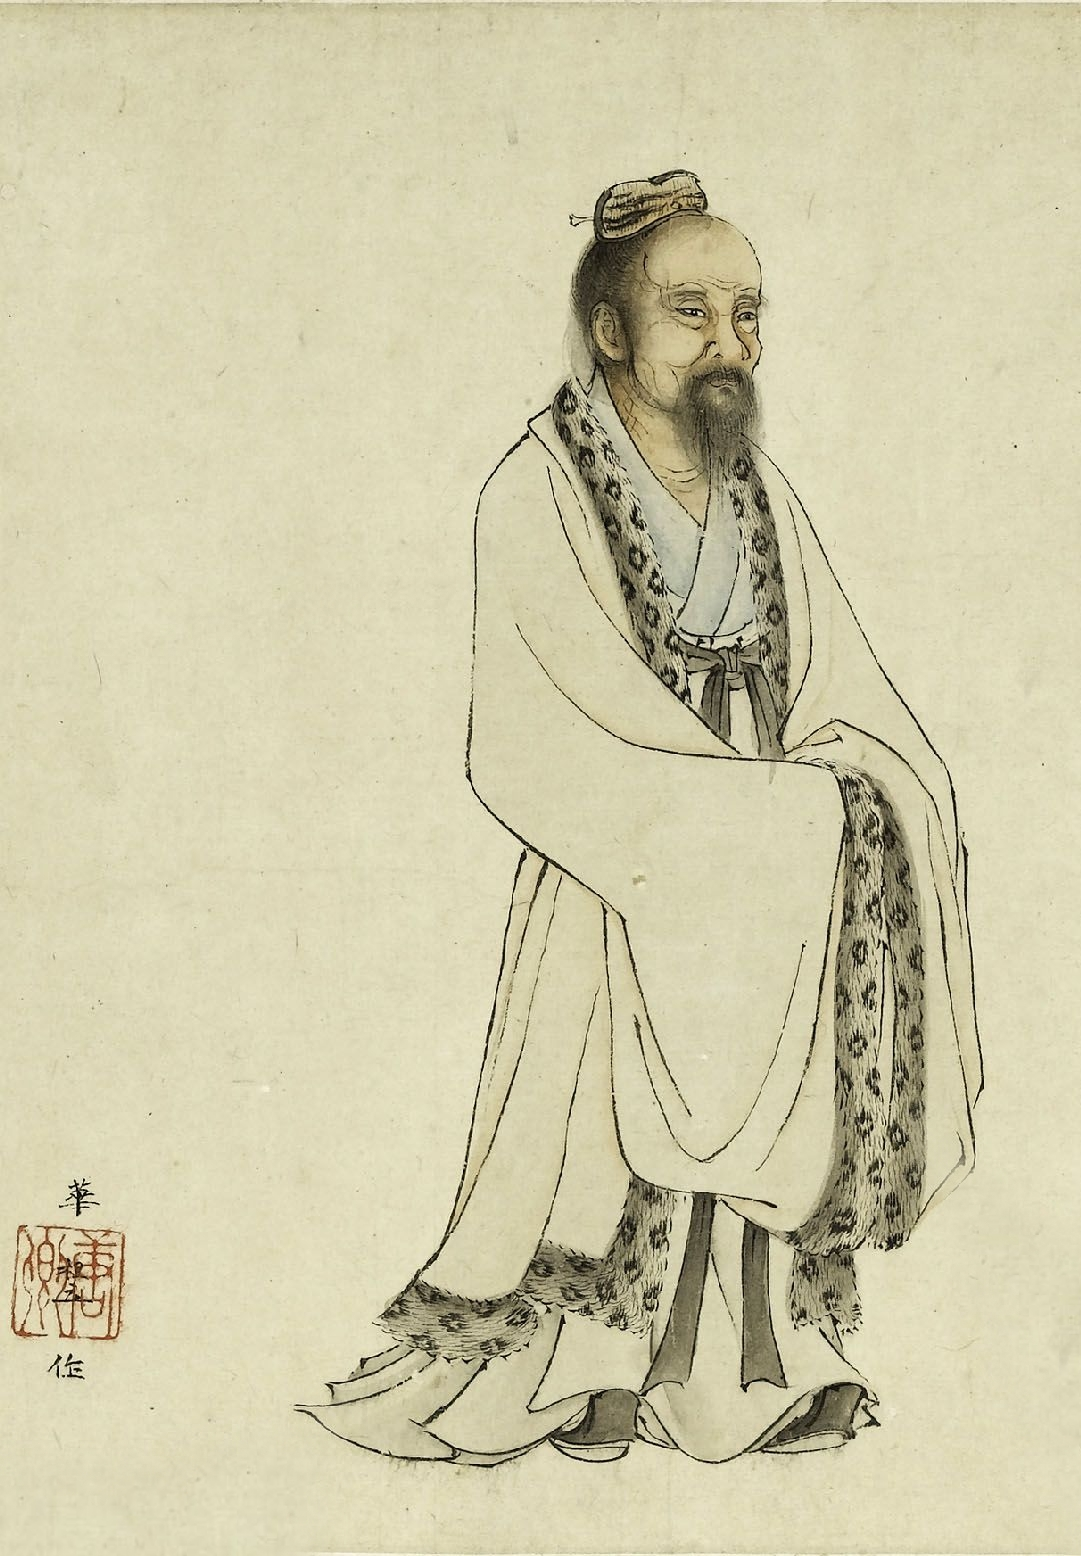
\includegraphics[height=0.7\textwidth]{../Figures/ZhuangZi.jpg}
    \caption{庄子像。元华祖立作。}
  \end{figure}
  
  \newpage

  \linenumbers

庄子名周,蒙人,生平几无可考事迹。
其生卒年难考,但史传庄子与齐宣王、梁惠王同时,可知其大抵与孟子(372 BC-289 BC)同时。
庄子思想承接老子且更为成熟,且《南华经》常有涉及老子之寓言,可见庄子当在老子之后。
庄子之学大旨宗老子之言,承其“道”、“反”、“无为”、“守柔”等理论,而又进一步肯定观赏世界之生命情意,破形躯、认知、德性。
庄子可谓道家学说之大成者。

\section{薄形骸}
庄子之自我境界在情意,为观赏之自我,系纯粹之生命境趣。
而情意往往与形躯混为一谈,难以区分。
盖人容易沉陷于形躯之感受,进而误以形躯为自我。
庄子欲破此谬误,遂有“薄形骸”之说。

\newline

为破形躯之境界,需先明其本质。
所谓形躯,实为一物理性存在之过程。
形躯之出现,系由一组条件所决定,而后遂有一存在历程。
此出现及存在即常识所谓之“生”。
而“死”为形躯存在之终点。
形躯之灭坏,其根本原因系万物之流变不息。
《南华经·至乐》载:

\textit{庄子妻死,惠子吊之,庄子则方箕踞鼓盆而歌。惠子曰:“与人居 ,长子、老、身死,不哭亦足矣,又鼓盆而歌,不亦甚乎!”庄子曰 :“不然。是其始死也,我独何能无概!然察其始而本无生;非徒无 生也,而本无形;非徒无形也,而本无气。杂乎芒芴之间,变而有气 ,气变而有形,形变而有生。今又变而之死。是相与为春秋冬夏四时 行也。人且偃然寝于巨室,而我噭噭然随而哭之,自以为不通乎命, 故止也。”}

民间传说庄子夫妻不和,大抵出自此则。
然此则意在薄形骸,言形躯之出现、存在、灭逝、转化皆物之流转变化,合乎物之规律。
总之,形躯实为一“物”。

\newline

然而自我并非万物之一,乃超越物质世界之主体,故形躯绝不等同于自我。
自我乃万物之外一超越主体,不受万物之影响。
《南华经·德充符》云:


\textit{死生亦大矣,而不得与之变;虽天地覆坠,亦将不与之遗;审乎无假而不与物迁,命物之化而守其宗也。}

此即言自我之主体超然物外,不为客观事物之转移而转移。
形躯与万物一同流转,其存在与否与自我之存在无干。
换言之,自我独立于万物之外,独立于形躯之外。

\newline

更进一步,形躯之存在往往干扰对自我之认知。
盖自我在自然历程中偶得一形躯,而人溺于形躯之感官感受,遂以形躯为自我,不知自我非物而形躯为物之道理。故《南华经·大宗师》云:

\textit{夫大块载我以形,劳我以生,佚我以老,息我以死。}

此非劝人自杀也。
生死本系形躯之成毁,系万物流变之一例,实与自我无关。
形躯之存在可阻碍自我之认知,可破坏形躯亦于事无补。
况且生死本一自然历程,强行打断并无益处,实属没事找事,吃饱了撑的。
自然而生便生,自然而死便死,无需为之苦恼。
换言之,纠结生死,以为破坏阻碍认知自我之形躯可有助于认知自我,本就是不知自我之表现。
若知自我之真意,则不自系于形躯,不执着于生死。
故《南华经·大宗师》云:

\textit{古之真人,不知说生,不知恶死。}

\section{泯是非}
庄子亦否定认知,不承认知识之地位,破坏知识之真伪标准,此即所谓“泯是非”。
现就此加以论述。

\newline

“泯是非”之第一论证基于知识自身之局限性。
任一项知识,皆为可补充、可修正者,并无绝对性。
故理论知识均为未完成者,则其所作肯定或否定之根基不牢,故无绝对性,属于成见,不能与绝对之真伪相符。
换言之,由认知活动获得理论知识固然是一成就,但由此生出一局限,使得真我蔽隐不显。
更进一步,欲破除此类成见,需使自我不溺于其中,不陷入是非之争执,而得以超越认知之迷雾,生一超经验之观悟,方可明一非认知之真正自我。
此观悟不由认知活动中生,而是自我之直接发用。
盖认知活动自有限制,不能显现真相,反为自我之累。
自我沉溺于认知活动,则永远只能于各种限制下构造理论,无法得悟。

\newline

第二论证基于知识之对立。首先,理论知识具有封闭性。譬如以一概念甲为基础,可构建一套理论体系,则此体系下一切存在皆以甲概念为依据;反之亦可以概念非甲为基础,构建另一套理论体系,则此体系下一切存在皆以非甲概念为依据。此为超越甲和非甲后所知之观念。若溺于甲之理论体系,则不见非甲;若溺于非甲之理论体系,则不见甲。由此可见此种概念系统之封闭性。这种封闭性使得两套理论孰是孰非无从论起。据于“甲”自然非“非甲”,据于“非甲”自然非“甲”,欲从中分辨是非自然无有意义,则认知之地位被否定矣。更进一步,甲和非甲互为矛盾,但彼此又互相依存。若不设一概念甲,则其反面概念非甲便无从谈起,反之亦然。甲和非甲,两套理论体系相反相成,彼此互为排斥,故有此消彼长之态势。可见认知所得理论系统不过概念游戏而已,彼此无本质区别,断非真我。最后,甲和非甲之对立,乃是认知活动强加区分,而非客观之存在。一旦超越此种对立,则对立双方皆无所依据,皆无价值矣。换言之,需超越此类“是”与“非”之对立,抛弃知识之迷障,方见最终真相,知认知绝非真我。
第三论证基于认知与经验世界之关系。一切判断和认知均需要一定之条件而成立,此等条件是基于经验事物。经验规律之呈现需要对于对客观事物之认知,而自我在此过程中起绝定性作用。事物之所以如此,并非客观存在即是如此,而是自我之认知活动将事物视为如此。故某物是如此,或不是如此,皆源于认知。可见,认知不见物之真正本质,只会产生幻象,令人以为某物是如此。由认知之幻象导致对不同物之间的区别,遂生判断。此种判断自然亦是幻象,毫无价值可言。更进一步,不同人的认知过程不尽相同,对同一物遂生不同判断,进而有辩议。然各人之判断皆源于各人之认知,皆不见物之本质,故辩议不足以定是非。反之,若能超越认知,便可摆脱认知所产生的关于事物之幻象,将不同事物视为等同,知其皆为“物”也,则明是非真伪之判断并无价值。可见,认知断非真正之自我。
至此作一总结。第一,知识自有其局限性,自我不应困于其中。第二,由知识系统之对立,推知互相反对之理论之封闭性及循环消长,进而否定认知之价值。第三,认知产生的对经验事物的知识皆为幻象,本无价值可言。综上,认知境界亦非自我之境界。

\section{文化与罪恶}
庄子论文化之真相,兹可作为“泯是非”之第四论证,然亦涉及德性之否定。盖所谓文化,可概括为对客观物质世界之知识以及人之道德伦理规范,前者系认知之领域,而后者系德性之领域。《南华经·胠箧》谓:
将为胠箧探囊发匮之盗而为守备,则必摄缄藤,固扃鐍,此世俗之 所谓知也。然而巨盗至,则负匮揭箧担囊而趋,唯恐缄藤扃鐍之不 固也。然则乡之所谓知者,不乃为大盗积者也?
此节以胠箧为喻,否定文化之价值。文化之发展本为消除罪恶,然文化愈加发展,罪恶亦愈发展。文化发展成果或能防止低级简单的罪恶,一如“摄缄藤,固扃鐍”可以防备低级盗贼。然而文化不但不能阻止高级复杂之罪恶,反而为之利用,一如“摄缄藤,固扃鐍”反而方便巨盗“负匮揭箧担囊而趋”。不唯技术可为罪恶利用,一切道德规范亦是如此。故《南华经·胠箧》又云:
故跖之徒问于跖曰:“盗亦有道乎?”跖曰:“何适而无有道邪?夫妄意室中之藏,圣也;入先,勇也;出后,义也;知可否,知也;分均,仁也。五者不备而能成大盗者,天下未之有也。”由是观之,善人不得圣人之道不立,跖不得圣人之道不行。天下之善人少而不善人多,则圣人之利天下也少而害天下也多。故曰:唇竭则齿寒,鲁酒薄而邯郸围,圣人生而大盗起。掊击圣人,纵舍盗贼,而天下始治矣。
道德规范可为善人所用,亦可为恶人所用,可见道德不足以消除罪恶。盖德性与认知均系中立性技术,自身无所谓善恶,可以用之为善,亦可用之为恶。可见,庄子否定认知和德性之价值。

\section{胜物}
现论庄子所肯定之境界及对德性之进一步否定,兹先观“胜物”。
“胜物”指不受外物支配,即自我不役于外物,包含不受形躯之局限,强调自我之主宰性。庄子以为自我之主宰表现于生命中,应使生命不作任何意义之工具。由此则德性之价值复破矣。盖孔孟贵人之德性,以为社会中人人皆有其“名”,进一步遂有其需完成义务权利。各人皆应履行各人之权利义务,完成其道德理分。依庄子,此即将生命用作实现道德意义之工具,自我陷溺于道德,而真我遭到遮蔽。
庄子反对以生命追求某种意义,认为此实系将生命视为一工具,阻碍真实自我之显现。故一切价值,于愚昧庸俗之人,固是价值;于明道至人,则是自我之害。“有用”必“被用”,既“被用”,则丧失自我,沦为工具矣。此即庄子论“无用之大用”之含义:“无用”即不追求任何意义或价值,“大用”即由“无用”显现真实之自我。
自我不应追求任何价值,则自我应当如何看待种种价值?换言之,自我对于非我之世界,应当持何种态度?此为文化之一甚大问题。盖儒学贵德,以道德为自我,致力于将世界置于道德之支配,遂有“化成世界”之态度。希腊哲学传统贵知,以认知为重,致力于认知世界之根本规律;更进一步,规律既可知,自然可为人所用,由此遂生“征服世界”之态度。佛家视存在本身为一恶,以自我陷溺于存在世界为苦,致力于将自我从世界中剥离,遂有“逃离世界”之态度。道家反对自我陷于外物,亦有逃离世界之倾向。然而老庄并不视存在本身为恶,故与佛家终为殊途。
依庄子,存在固非一罪,自我无需从存在终逃离,而应当不作为一经验存在参与经验事物之活动,安然观赏万物各依道运行,于经验界既无所追求,亦不需有所追求。如此,自我观赏流变之世界,既无所求,亦无所执,故形躯、知识、道德是非皆不系于心。自我顺物自然,观赏自得,成情意之境界。

\section{养生}
庄子论养生,所养者即为情意之观赏能力。兹以庖丁解牛之寓言释之。《南华经·养生主》载:
庖丁为文惠君解牛,手之所触,肩之所倚,足之所履,膝之所倚,砉然响然,奏刀騞然,莫不中音。合于《桑林》之舞,乃中《经首》之会。文惠君曰:“嘻,善哉!技盍至此乎?”庖丁释刀对曰:“臣之所好者道也,进乎技矣。始臣之解牛之时,所见无非全牛者;三年之后 ,未尝见全牛也;方今之时,臣以神遇而不以目视,官知止而神欲行 。依乎天理,批大郤,导大髋,因其固然。技经肯綮之未尝,而况大軱乎!良庖岁更刀,割也;族庖月更刀,折也;今臣之刀十九年矣,所解数千牛矣,而刀刃若新发于硎。彼节者有间而刀刃者无厚,以无厚入有间,恢恢乎其于游刃必有余地矣。是以十九年而刀刃若新发于硎。虽然,每至于族,吾见其难为,怵然为戒,视为止,行为迟,动刀甚微,謋然已解,如土委地。提刀而立,为之而四顾,为之踌躇满志,善刀而藏之。”文惠君曰:“善哉!吾闻庖丁之言,得养生焉。”
此故事以牛喻经验世界,以刀刃喻自我,解牛即自我与经验世界之关系,而故事之重点在于如何使刀不伤。苟谓世上本无牛可解,刀刃自然不伤,此为佛学之舍离;谓牛应解,刀应于解牛,伤与不伤不足为论,则为儒家之化成。而庄子所重视者,乃是刀刃之不伤。纠结于是否有牛、牛是否应解以及是否应以刀刃解牛皆无价值。既不以牛为累,亦不以为刀刃应当用于解牛,但求自然游刃解牛。换言之,庄子所欲肯定者,为不以经验世界限定自我,亦不认为自我需完成某些价值,但求自我顺物之自然,超越经验世界,观赏万物之流变不息。此为养生之真意。其所养者乃情意之境界,自我不作逃离世界,不求完成价值,仅只观赏万物。

\section{逍遥游}
至此,可对庄子之学说作一总结。庄子以为形躯不足贵,认知无价值,德性没意义,文化只会滋生罪恶。其所肯定者,唯有一逍遥自在、观赏万物之自我。此一境界,超越经验世界,不作逃离,不执于物,不求任何价值之完成,仅自由观赏经验世界之运行。故《南华经·逍遥游》论此境界谓:
至人无己,神人无功,圣人无名。
  
\end{document}